% To familiarize yourself with this template, the body contains
% some examples of its use.  Look them over.  Then you can
% run LaTeX on this file.  After you have LaTeXed this file then
% you can look over the result either by printing it out with
% dvips or using xdvi.


\documentclass[twosided]{article}
\setlength{\oddsidemargin}{0.25 in}
\setlength{\evensidemargin}{0.25 in}
\setlength{\topmargin}{-0.6 in}
\setlength{\textwidth}{6.5 in}
\setlength{\textheight}{8.5 in}
\setlength{\headsep}{0.75 in}
\setlength{\parindent}{0 in}
\setlength{\parskip}{0.1 in}

%
% ADD PACKAGES here:
%

\usepackage{amsmath,amsfonts,graphicx,algorithm,caption}
\usepackage{cite}

%\usepackage{algpseudocode}
%\usepackage{natbib}
\usepackage[document]{ragged2e}
\usepackage{graphicx} %package to manage images
\usepackage{mathtools}
\usepackage{algorithm,algorithmic}
%\usepackage[options ]{algorithm2e}
\usepackage{amssymb,multirow,array,tikz}
\usepackage{epsfig,amsthm}
\usepackage{blkarray}
\usepackage{commath}
\usepackage[english]{babel}
\usepackage{url}
%\usepackage[utf8x]{inputenc}
%\usepackage[T1]{fontenc}


%
% The following commands set up the lecnum (lecture number)
% counter and make various numbering schemes work relative
% to the lecture number.
%
\newcounter{lecnum}
\renewcommand{\thepage}{\thelecnum-\arabic{page}}
%\renewcommand{\thesection}{\thelecnum.\arabic{section}}
\renewcommand{\thesection}{\thelecnum.\arabic{section}}
\renewcommand{\theequation}{\thelecnum.\arabic{equation}}
\renewcommand{\thefigure}{\thelecnum.\arabic{figure}}
\renewcommand{\thetable}{\thelecnum.\arabic{table}}
\makeatletter
%\def\BState{\State\hskip-\ALG@thistlm}
%\makeatother
%
% The following macro is used to generate the header.
%
\newcommand{\lecture}[4]{
   \pagestyle{myheadings}
   \thispagestyle{plain}
   \newpage
   \setcounter{lecnum}{#1}
   \setcounter{page}{1}
   \noindent
   \begin{center}
   \framebox{
      \vbox{\vspace{2mm}
    \hbox to 6.28in { {\bf IE643: Deep Learning : Theory and Practice
		\hfill July-Dec 2021} }
       \vspace{4mm}
       \hbox to 6.28in { {\Large \hfill Lecture #1: #2  \hfill} }
       \vspace{2mm}
       \hbox to 6.28in { {\it Lecturer: #3 \hfill Scribes: Your Name} }
      \vspace{2mm}}
   }
   \end{center}
   \markboth{Lecture #1: #2}{Lecture #1: #2}

   %{\bf Note}: {\it LaTeX template courtesy of UC Berkeley EECS dept.}

   {\bf Disclaimer}: {\it These notes have not been subjected to the
   usual scrutiny reserved for formal publications.  They may be distributed
   outside this class only with the permission of the Instructor.}
   \vspace*{4mm}
}
%
% Convention for citations is authors' initials followed by the year.
% For example, to cite a paper by Leighton and Maggs you would type
% \cite{LM89}, and to cite a paper by Strassen you would type \cite{S69}.
% (To avoid bibliography problems, for now we redefine the \cite command.)
% Also commands that create a suitable format for the reference list.
%\renewcommand{\cite}[1]{[#1]}
%\def\beginrefs{\begin{list}%
%        {[\arabic{equation}]}{\usecounter{equation}
%         \setlength{\leftmargin}{2.0truecm}\setlength{\labelsep}{0.4truecm}%
%         \setlength{\labelwidth}{1.6truecm}}}
%\def\endrefs{\end{list}}
%\def\bibentry#1{\item[\hbox{[#1]}]}

%Use this command for a figure; it puts a figure in wherever you want it.
%usage: \fig{NUMBER}{SPACE-IN-INCHES}{CAPTION}
\newcommand{\fig}[3]{
			\vspace{#2}
			\begin{center}
			Figure \thelecnum.#1:~#3
			\end{center}
			}

% Use these for theorems, lemmas, proofs, etc.
\newtheorem{theorem}{Theorem}[lecnum]
\newtheorem{lemma}[theorem]{Lemma}
\newtheorem{proposition}[theorem]{Proposition}
\newtheorem{claim}[theorem]{Claim}
\newtheorem{corollary}[theorem]{Corollary}
\newtheorem{definition}[theorem]{Definition}
%\newenvironment{proof}{{\bf Proof:}}{\hfill\rule{2mm}{2mm}}

% **** IF YOU WANT TO DEFINE ADDITIONAL MACROS FOR YOURSELF, PUT THEM HERE:
%\newcommand{\R}{\mathbb{R}}

\begin{document}
%FILL IN THE RIGHT INFO.
%\lecture{**LECTURE-NUMBER**}{**DATE**}{**LECTURER**}{**SCRIBE**}
\lecture{2}{Topic of lecture (30-July-2021)}{P. Balamurugan}{Your Name}
%\footnotetext{These notes are partially based on those of Nigel Mansell.}

% **** YOUR NOTES GO HERE:

% Some general latex examples and examples making use of the
% macros follow.  
%**** IN GENERAL, BE BRIEF. LONG SCRIBE NOTES, NO MATTER HOW WELL WRITTEN,
%**** ARE NEVER READ BY ANYBODY.



\section{Some topic}
Discuss about the topics discussed in class in your own words. If you use text from some other source, cite them. Example of citation: Perceptron is described in \cite{Rosenblatt58theperceptron, rosenblatt1957perceptron}.

Write clearly about each topic discussed in class. Be complete. Be concise. Be comprehensive. 

\section{Example Section: Biological Motivation of Perceptron}

The perceptron proposed by Rosenblatt \cite{Rosenblatt58theperceptron} was motivated using a neuron present in human and other mammalian nervous systems. A human neuron contains a nucleus, an axon and dendrites (see Figure \ref{fig:neuron}). The dendrites connect one neuron to other and help in the transmission of impulses between neurons. The nucleus processes the impulses and depending on biological considerations, the neuron either becomes activated and transmits the processed impulses to a subset of the adjoining neurons or remains inactive. A similar idea is used in perceptron. Perceptron accepts $d$ inputs of the form $+1$ or $-1$ and then computes a weighted sum of the inputs using weights denoted by $w_1, w_2,\ldots, w_d$ and compares the weighted sum to a threshold $\theta$ and outputs either $+1$ or $-1$ indicating that the perceptron is active or inactive respectively. This is illustrated in Figure \ref{fig:perceptron}. 

\begin{figure}[!h]
 	\centering
 	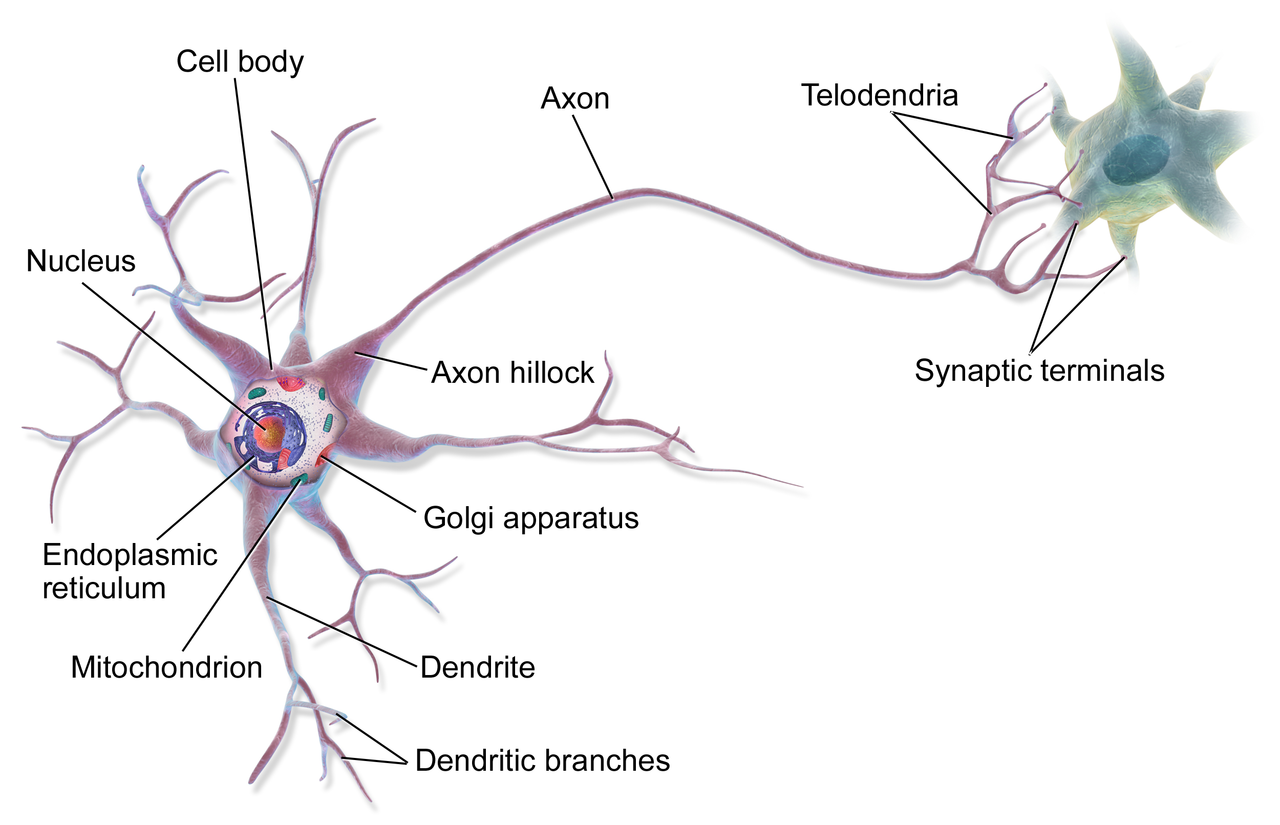
\includegraphics[width=0.5\textwidth]{neuron.png}
 	\caption{Structure of a neuron \cite{neuron_wikipedia_article} (\textbf{Note:} cite source of the figure if it is not your own.)}
 	\label{fig:neuron}
\end{figure}



\subsection{Here's a subsection}

\begin{theorem} This is how you can write a theorem. 
\end{theorem}
\begin{proof}
	A sample proof of $|a+b| \leq |a| + |b|, \forall a,b \in \mathbb{R}$.
	
	First note that 
	\begin{align}
	|a||b|\geq ab, \forall a,b \in \mathbb{R}. \label{first_result}
	\end{align}
	This can be proved by considering the following four cases: (without loss of generality assume $a\neq 0, b\neq 0$)
	\begin{itemize}
		\item $a>0,b>0: \implies |a|=a, |b|=b$. Hence $ab = |a||b|$. 
		\item $a<0,b<0: \implies |a|=-a, |b|=-b$. Hence $|a||b| = (-a)(-b)=ab$.  
		\item $a<0,b>0: \implies |a|=-a, |b|=b$. Hence $|a|\geq a$. Therefore, $|a||b| \geq ab$.
		\item $a>0,b<0: \implies |a|=a, |b|=-b$. Hence $|b|\geq b$. Therefore, $|a||b| \geq ab$.
	\end{itemize} 
	Also from the above arguments, note that
	\begin{align}
	|a|^2 = a^2, \ \forall  a \in \mathbb{R}. \label{second_result}
	\end{align} 
	Now consider $(|a|+|b|)^2$. We get
	\begin{align}
	(|a|+|b|)^2 & = |a|^2 + |b|^2 + 2|a||b| \nonumber \\
	& = a^2 + b^2  + 2|a||b| \text{  (Using \eqref{second_result})} \nonumber \\
	& \geq a^2 + b^2  + 2ab \text{  (Using \eqref{first_result})} \nonumber \\
	& = (a+b)^2. \label{last_step}		
	\end{align}
	Thus we have $(|a|+|b|)^2 \geq (a+b)^2$. 
	Now taking square root on both sides, we get the required result $(|a|+|b|) \geq |a+b|$.  
	
	Hence the required proof.
\end{proof}


\section{Template for algorithm}

Write an algorithm using the following template. 

\begin{algorithm}[H]
	\caption{A sample algorithm}
	\begin{algorithmic}[1]
		\STATE \textbf{Input:} Here comes the input of the algorithm. 
		\STATE \textbf{Initialize:} Include any initialization. 
		\FOR{$k=1,2,\ldots$}
		\STATE Here is the computation within the loop. 
		\ENDFOR
		\IF{some condition}
		\STATE Do action 1
		\ELSE
		\STATE Do action 2 
		\ENDIF
		\WHILE{some condition is true}
		\STATE Perform some computation
		\ENDWHILE
		\STATE \textbf{Output:} Write the output here. 
	\end{algorithmic}
\end{algorithm}

\begin{lemma}
	This is how you can state any lemma
\end{lemma}


\begin{definition}
	Example to write any definition
\end{definition}

\begin{claim}
	Claim can be stated like this.
\end{claim}
\begin{figure}[!h]
	\centering
	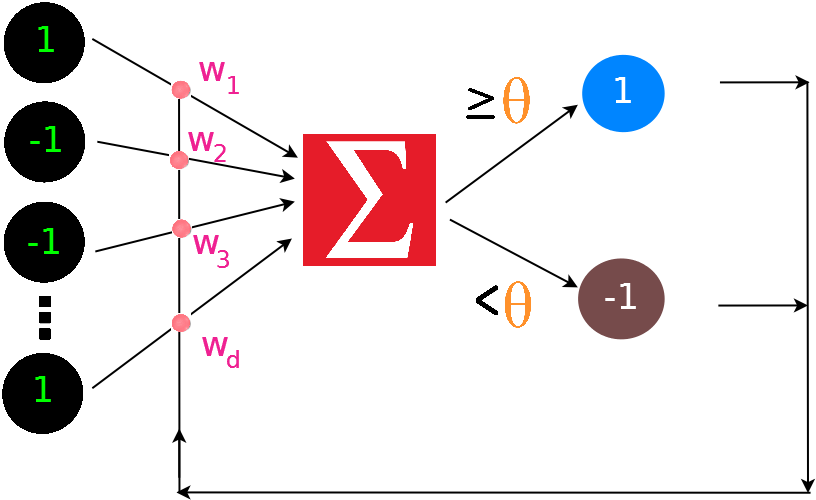
\includegraphics[width=0.5\textwidth]{perceptron.png}
	\caption{Example to add a figure}
	\label{fig:perceptron}
\end{figure}

Once you've inserted the figure, you can refer to it as figure \ref{fig:perceptron}


\section{Some general guidelines for scribing}

\begin{enumerate}
	\item Please note that slides will not be made available until scribes are ready. Only lecture video will be available. Please watch the video carefully and describe all the points discussed in the video. 
	\item Write all text yourself. Do not copy and paste text from some other resource. Copied material with a citation is also not allowed.  
	\item Prepare images yourself. You can use images in the lecture videos (you can use capture tools like vlc media player to take a screenshot of an image from video) but it would be great if you can prepare your own images and add to the scribes.  
	\item If you are forced to include some figure from some other resource, please include appropriate source (or website) from which the figure was taken. See e.g. Figure \ref{fig:neuron}.
 	\item  If there is something which you did not understand in the class, try to understand and be clear before writing. You can always discuss with the instructor or the TAs. 
	\item Try your best that these notes are useful to others.	
	\item Do not be informal in your notes!
	\item Add the references in the bibtex file called demo.bib in this folder. Use them to cite the appropriate references. Examples of how to cite a paper are given in the sections above.  
	\item Do not miss any topic covered in class. 
\end{enumerate}
	

% Add the "demo.bib" file in the same folder. The following command will add references to your scribe. Change the quick build settings in the following way. 
%Options -> Configure Texmaker -> Quick Build -> Select the PdfLatex+Bib(la)Latex+PdfLatex(x2)+ViewPdf option


\newpage
\bibliographystyle{plain}
\bibliography{demo}{} % Because the file name is demo.bib
%\nocite{*}
\end{document}

